\documentclass{article} % For LaTeX2e
% We will use NIPS submission format
\usepackage{nips13submit_e,times}
% for hyperlinks
%\usepackage{hyperref}
\usepackage{url}
% For figures
\usepackage{graphicx} 
\usepackage{subfigure} 
% math packages
\usepackage{amsmath}
\usepackage{amsfonts}
\usepackage{amsopn}
\usepackage{ifthen}
\usepackage{natbib}
\usepackage{color}
\usepackage{float}
\usepackage{placeins}
\usepackage{geometry}
\usepackage{listings}

\title{Project-II by Group Istanbul}

\author{
Johan Droz\\
EPFL \\
\texttt{johan.droz@epfl.ch} \And
Arseniy Zaostrovnykh\\
EPFL \\
\texttt{arseniy.zaostrovnykh@epfl.ch}
}

% The \author macro works with any number of authors. There are two commands
% used to separate the names and addresses of multiple authors: \And and \AND.
%
% Using \And between authors leaves it to \LaTeX{} to determine where to break
% the lines. Using \AND forces a linebreak at that point. So, if \LaTeX{}
% puts 3 of 4 authors names on the first line, and the last on the second
% line, try using \AND instead of \And before the third author name.

\nipsfinalcopy 

\newcommand{\todo}[1]{}
\renewcommand{\todo}[1]{{\color{red} TODO: {#1}}}

\begin{document}

\maketitle

\begin{abstract}
In this report we describe our results for the second project of the 2015 PCML class.
Our goal is to design a system that, given an image, is able to recognize three kinds of object in it.
We tried to improve the accuracy of the system by experimenting with different methods.

\end{abstract}

\section{Introduction}

The problem of classifying images is a hot topic on which most of the big IT companies are working on.
Google, Tesla and probably other companies are building autonomous car, that has to be able to recognize in real-time object such as other vehicles, pedestrians, traffic lights, roadsigns...
Thousands, even millions of images are uploaded and automatically processed in social networks every days.

The system we have to design is simpler than the two previous example, in the sense that there are only 4 categories of objects. Nevertheless, the task of recognizing an object in an image is still complex for many reasons.
Firstly an image has high dimension, which make the job of building, tuning and testing a model complicated.
Secondly two very similar images can have different label.
Take for example the images in figure \ref{fig:car_tire} and \ref{fig:tire} look similar, but they have different label. The first one is labeled as "Car" and the second fall into the "Other" categorie. Moreover the images in figure \ref{fig:car_tire} and \ref{fig:car} don't have a lot in common, but they are both labeled as car.
Sometimes the object is cropped: only a part of it appear in the image. The object can be hidden by another object, or several objects are appearing in the same image, which make it difficult to distinguish the one we are interested in.

For this project the ML methods we can try are limited. The code submitted has to reproduce the results and cannot be larger than 20MB. So we cannot experiment with various toolboxes without violating this limit.
And for the testing set only the HOG and CNN features are provided, not the original images which has for consequence that we cannot extract other features ourselves but have to work only with these two.

\begin{figure}[!t]
	\centering
	\subfigure[Car (label = 2)]{\label{fig:car_tire}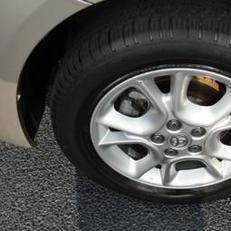
\includegraphics[width=0.3\textwidth]{figures/train00368.jpg}}
	\subfigure[Tire (label = 4)]{\label{fig:tire}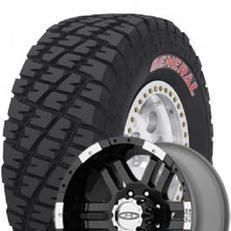
\includegraphics[width=0.3\textwidth]{figures/train00942.jpg}}
	\subfigure[Another car (label = 2)]{\label{fig:car}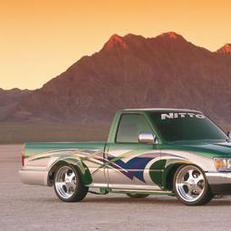
\includegraphics[width=0.3\textwidth]{figures/train04139.jpg}}
	\caption{Some sample from the training set}
\end{figure}

\section{Data Description}

The system we have to design has to be able to classify images based on what object they contain. 
There are 4 classes: the image can contain an airplane, a car, a horse or neither of them.

A training set containing either color or grayscale images of size 231x231 is given. It contains 6000 images, each associated with a label and two sets of features: the Histogram of Oriented Gradients (HOG) and the OverFeat ImageNet CNN Features.
Out of these 6000 images there is 964 airplanes, 1162 cars, 1492 horses and 2382 other objects.
Unfortunately we don't know if the testing data follows the same distribution.

For acceleration of the experiments, we considered the ways to reduce the number of features. 

One ways is to scale down the input images. However, this affects only the HOG features, as CNN represents the neural network weights and does not depend on the number of pixels in the image.

The CNN feature array seems very sparse. However an investigation shown that each feature(except for the last one) is nonzero for at least 20 images in the train set.

Other way is to find correlations in that matrix. no way: number of features ~36000, number of data-points 6000 -> matrix rank is going to be <= 6000 => there are a lot of linear combinations of the columns.

Note: move from small-pics to the originals require a complete recalibration of SVM meta-parameters

Note: hard-negative mining

Note: the best-optimized SVM(HOG) gives 0.1734 test BER and 0.0554 train BER on 3-fold cross validation.

Averaging all the boxes into a single histogram does not work.

\paragraph{HOG feature} HOG is widely use in computer vision. 
The basic idea is that the shape and appearance of an object is often well characterized by the distribution of local intensity gradients or edge directions \cite{hog}.
Figure \ref{fig:image_car} and \ref{fig:hog} shows respectively an image form the training set and a visualization of its HOG feature.
And in fact, the shape of the car is recognizable in the HOG visualization.

\paragraph{CNN features} Features extracted from the OverFeat convolutional neural network (CNN).

\begin{figure}[!t]
	\centering
	\subfigure[Training image]{\label{fig:image_car}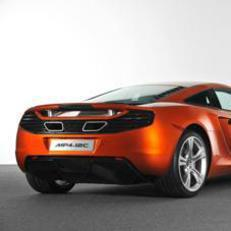
\includegraphics[width=0.4\textwidth]{figures/train00003.jpg}}
	\hspace{10pt}
	\subfigure[HOG feature]{\label{fig:hog}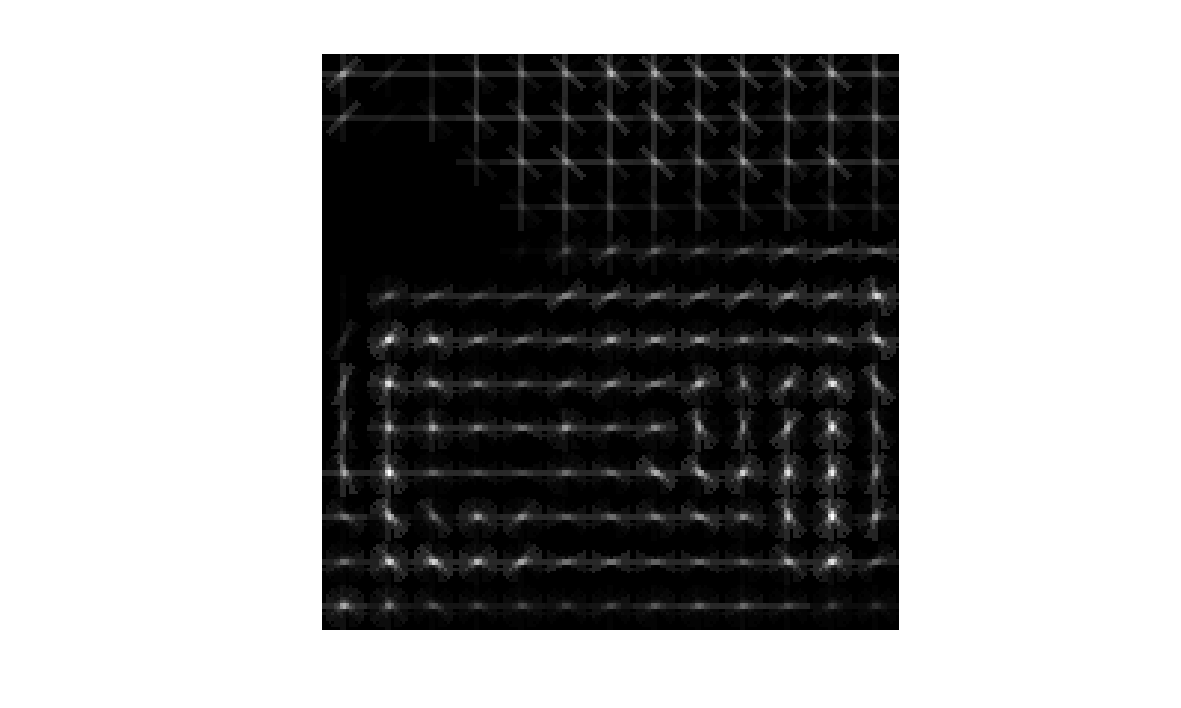
\includegraphics[width=0.4\textwidth]{figures/hog.pdf}}
	\caption{Visualization of the HOG feature}
\end{figure}

The testing set contains only the HOG and CNN features and not the images from which those feature are extracted.
As a consequence we should focus on optimizing the classification based on these two set of features, and not trying to extract different one.
The testing set contains 11'453 samples and we have to submit two predictions: a binary prediction, that is whether the image contains either a car, a plane or a horse, or neither of them and a multiclass 
prediction, where we predict the object present in the image.

\paragraph{Training data}

I do not think that a horse, a car and an airplane share any common structure, so it its reasonable to do binary prediction based on the multiclass prediction. Simply:
y = (y ~= 4)  -- if classifier have not found any of these three, answer no.

Each class should be detected separately, of course:

\begin{lstlisting}

if (y_{horse} == 1) y = 1
else if (y_{car} == 1) y = 2
else if (y_{airplane} == 1) y = 3
else y = 4
end
\end{lstlisting}

We should think how do we handle disputed cases (e.g. $y_{horse}$ == 1 and $y_{car} == 1$). we may train 3 additional classifiers for each of those (if we get enough cases for it).

\section{Data visualization and basic exploratory data analysis}


\subsection{Performance measures}

\section{Predict test data}
This section describes the different Machine Learning (ML) methods and models used to classify the images. 
First we detail the performance measure, then the classification methods.
We experimented with both binary and multiclass classification.
We chose to focus on improving multiclass classification as much as we can, and from those results, we can easily derive the binary predictions.


\subsection{Cross-Validation}

K-fold and Balanced Error Rate (BER) are used to measure the performance of the classification methods.
K-fold return an unbiased estimate of the error by randomly partitioning the data into K groups, training on K-1 group and testing on the remaining one. This is done on all K sets.
The parameter K is not easy to set for this project. 
We want a K that split the training and testing set with a good proportion, that is there is enough data in the training set to train a neural network, SVM or a random forest while at the same time having a testing set large enough to estimate the BER.
A problem here is that for each fold we have to train the model, which is time consuming. 
We used a K equal to 3, because for larger K we waste too much time training the model.

\subsection{Convolutional Neural Network}
The file named \emph{imageClassificationExample.m} given in the project website use a simple neural network (NN) from the \emph{DeepLearnToolbox}.
In the example, this NN is trained on the HOG features and give a BER of 29.32\% with 3-Fold Cross validation. Note that the others parameters are still set to their default values, that is the number of epochs is 20, the batch size 100, the learning rate 2.

We tried to train the NN with the CNN features and the same configuration, and this time the BER is 12.73\%.
The next step is trying to find optimal values for the parameters with a grid search. As the NN takes quite a long time to train, we cannot afford to do a grid search with too many parameters.
Here we 


\subsection{Random Forests}
We saw in class that Random Forests (RF) are one of the last techniques capable to compete with Neural Networks.
As a consequence, we chose to experiment with them to try to outperform our firsts results.

Random forests choose randomly a subset of input variables to build many trees and reduce the variance of the output by taking the average of many outputs.

Here we use the matlab function named \emph{TreeBagger}. We set the number of trees to 300, this value was determined with grid search.
We obtain a BER of 12.57\% with 3-fold cross validation. Table \ref{tbl:errClassNotBal} shows the predictions error for each class. Take the first line as example. The true class is Airplane and there is $N_c$ sample in it. The following columns shows what the random forest predicted.
Here we notice that the majority of error is because the method put an image in the categorie Other when it is actually another one.
This is maybe because of the class imbalance during the training of the model. Indeed we mention earlier that there is 6000 images: 964 airplanes, 1162 cars, 1492 horses and 2382 other objects.

The next step is to train the model with the same proportion of images in each class, by randomly deleting sample in the classes with more data. Ideally, we would prefer adding images in the class with less samples, so we don't reduce our training set but increase it.
So we end up with a training set containing 964 images for each class. 
We obtain a BER of 9.68\%. Table \ref{tbl:errClassBal} shows the BER for each class.

\begin{table}[!htb]
	\centering
		\begin{tabular}{|c|c|c|c|c|c|c|}
			\hline Class & $N_{c}$ & Airplane & Car & Horse & Other & BER \\ 
			\hline Airplane & 332 & 267 & 7 & 0 & 58 & 19.58\% \\ 
			\hline Car & 397 & 1 & 375 & 4 & 17 & 5.54\% \\ 
			\hline Horse & 490 & 0 & 0 & 403 & 87 & 17.76\% \\ 
			\hline Other & 781 & 1 & 11 & 27 & 742 & 4.99\% \\ 
			\hline 
		\end{tabular} 
		\caption{Predictions error for each class with unbalanced training set}
		\label{tbl:errClassNotBal}
\end{table}

\begin{table}
	\centering
	\begin{tabular}{|c|c|c|c|c|c|c|}
		\hline Class & $N_{c}$ & Airplane & Car & Horse & Other & BER \\ 
		\hline Airplane & 310 & 293 & 5 & 2 & 10 & 5.48\% \\ 
		\hline Car & 349 & 12 & 325 & 4 & 8 & 6.88\% \\ 
		\hline Horse & 311 & 4 & 0 & 286 & 21 & 8.04\% \\ 
		\hline Other & 315 & 8 & 10 & 39 & 258 & 18.10 \% \\ 
		\hline 
	\end{tabular} 
	\caption{Predictions error for each class with balanced training set}
	\label{tbl:errClassBal}
\end{table}


\subsection{SVM}

Hard-negation mining.

Optimal parameter choice

\subsection{Ensemble classifier}


%\begin{figure}[!t]
%	\centering
%	\subfigure[Scatter plot of one input variable vs output]{\label{fig:scatter}\includegraphics[width=0.55\textwidth]{figures/X58vsY.pdf}}
%	\subfigure[Histogram of $\boldmath{y\_train}$]{\label{fig:histY}\includegraphics[width=0.4\textwidth]{figures/histY.pdf}}
%	\caption{Data analysis}
%\end{figure}



%\begin{figure}[!t]
%	\center
%	\includegraphics[width=0.8\textwidth]{figures/ridgeRegLoss.pdf}
%	\caption{Plot of the test and training error for ridge regression}
%	\label{fig:ridgeRegError}
%\end{figure}


\section{Summary}












\bibliographystyle{plain}
\bibliography{References.bib}

\end{document}
